\chapter{Preliminaries}

%-------------------------------------------------------------
%Here goes the introduction of transport between quantum dots. stil need to add important considerations like the smooth varying DOS. Not so discrete. 
%Assumption: 
%   1-Only the level immediately at the bottom of the fermi       level is considered
\section{Transport in Quantum Dots (QDs)}
Quantum mechanical effects are visible when the system size is of
the order of the de Broglie wavelength \citep[(1.1)]{bimberg_quantum_1999}
\[
\lambda_{f}=\frac{h}{\sqrt{3m_{\mathsf{eff}}k_{B}T}}
\]
 where $m_{\mathsf{eff}}$ is the electron effective mass in the crystal.
Since this mass can be much smaller than the free electron mass in
some semiconducting materials, size quantization effects can be observed
at system of sizes $\sim100\mbox{nm}$ \citep[2.1]{sindel_numerical_2005}.
A device confined in the three dimensions up to this length-scale
will present the behavior of a $0$D quantum system, which is what
we call a Quantum Dot (QD).\\

Nowadays there are several methods for manufacturing QDs \citep{bimberg_quantum_1999}.
One of them can be observed in \ref{QD} where 2 QDs are defined by
metallic gates on top of a semiconductor structure. Between the gates
a $2$-dimensional electron gas (2DEG) forms. A negative voltage is
applied at the top of gates $A,\ B,\ 1$ and $2$ such that the electron
gas is confined into the small electron droplets in the middle of
the gates. Furthermore, it is possible to control accurately the tunnel
barriers between the dots and the environment by setting appropriate
gate-voltages. This property is extremely useful since it allows us
to control the energy levels inside the QD and will take a huge relevance
in transport measurements. \\

\begin{figure}[h]
\centering
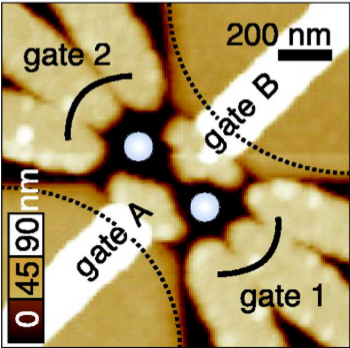
\includegraphics[scale=0.55]{IMAGES/QD-horizontal.png}\caption{Taken from \citep{holleitner_probing_2002}. Atomic force microscopy
picture of two coupled lateral QDs (bright central circles). A negative
voltage is applied at gates $A$,$B$,$1$ and $2$, which leads to
a partial depletion of the 2DEG.\label{QD}}
\end{figure}


The great advantage of QDs is that their spectrum looks pretty similar
to the spectrum of an atom, which is a discrete set of energy levels.
Indeed we can model an ideal single-electron QD as a quantum well
with a negative constant potential inside the dot . For example an
spherical quantum dot with radius $R$ will take the following Schr�dinger
Hamiltonian 

\[
H\Psi(r)=\left(\frac{\hbar^{2}}{2m^{*}}\nabla^{2}+V(r)\right)\Psi(r)\ ,\ \textrm{with }V(r)=\begin{cases}
-V_{0} & r<R\\
0 & r\geq R
\end{cases}.
\]


The 
the energy level spacing is  \citep[Equation (5.44)]{bimberg_quantum_1999}

\[
\delta E\propto\frac{1}{R^{2}}.
\]



%------------------------------------------------------------
\subsection{The Anderson Model}

For more electrons, due to the small spatial confinement, the coulomb
repulsion inside the dot is important. We also consider that the system is interacting. Hence, using the Hunds rule we know that
the energy levels should be filled from lower to higher energies with
two electrons with different spin at each state. Taking in account
all these interactions we can get to a second quantization QD-Hamiltonian
of the form \citep[(3.2)]{sindel_numerical_2005}

\[
H_{d}=\sum_{i\sigma}\epsilon_{di}d_{i\sigma}^{\dagger}d_{i\sigma}+\sum_{i}U_{i}\hat{n}_{i\uparrow}\hat{n}_{i\downarrow}+\sum_{\sigma\sigma',i\neq j}U_{ij}\hat{n}_{i\sigma}\hat{n}_{j\sigma'}-\mu_{B}gB\sum_{i}S_{i}^{z}+J\sum_{i\neq j}\mathbf{S}_{i}\cdot\mathbf{S}_{j}.
\]


Where $\sigma\in\{\uparrow,\downarrow\}$, $d_{i\sigma}^{\dagger}\left(d_{i\sigma}\right)$
is the dot creation(annihilation) operator,$\hat{n}_{i\sigma}:=d_{i\sigma}^{\dagger}d_{i\sigma}$
is the particle number, $\mathbf{S}_{i}$ is the spin-vector, $\epsilon_{di}$
is the energy of the $i^{\mbox{th}}$-level in the dot, $U_{i}$ is
the coulomb repulsion between electrons in the same energy level $i$,
$U_{ij}$ is the coulomb interaction between electrons in different
levels (And therefore smaller than $U_{i}$), \textbf{$B$} is an
applied magnetic field in the $\hat{z}$-direction and $J$ is the
term representing the Zeeman splitting. We now use that we can control
the energy levels of the QD by switching set the gate-voltage, such
that we only take in consideration one level in the QD. Taking this
assumption the dot Hamiltonian becomes \\

\begin{figure}[h]
\centering
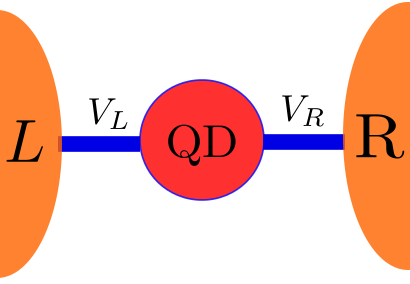
\includegraphics[scale=0.45]{IMAGES/QD_transport.png}\caption{\label{QD-transport}Transport measurement scheme in the QD. }
\end{figure}


\[
H_{d}=\sum_{\sigma}\epsilon_{d}d_{\sigma}^{\dagger}d_{\sigma}+U\hat{n}_{\uparrow}\hat{n}_{\downarrow}-\mu_{B}gBS^{z}.
\]


Since we are interested in implementing transport measurements through
the QD we need to link the dot to two metallic leads ($L$(left) and
$R$(right)) so that electron conduction can be performed (\ref{QD-transport}).
For this we can add two new hamiltonians in second quantization that
represent the energy of the electrons inside the leads $H_{lead}$
and the interaction between the leads and the quantum dot $H_{int}$.
These hamiltonians take the form 

\begin{eqnarray*}
H_{lead} & = & \sum_{\mathbf{k}\sigma l}\epsilon_{\mathbf{k}l}c_{\mathbf{k}\sigma l}^{\dagger}c_{\mathbf{k}\sigma l}\\
H_{int} & = & \sum_{\mathbf{k}\sigma l}V_{\mathbf{k}l}c_{\mathbf{k}\sigma l}^{\dagger}d_{\sigma}+V_{\mathbf{k}l}^{*}d_{\sigma}^{\dagger}c_{\mathbf{k}\sigma l},
\end{eqnarray*}


where $\mathbf{k}$ represents the possible crystal momentums in the
leads, $l\in\{L,R\}$, $c_{\mathbf{k}\sigma l}^{\dagger}(c_{\mathbf{k}\sigma l})$
creates(annihilates) an electron with momentum $\mathbf{k}$ and spin
$\sigma$ in the lead $l$, $\epsilon_{\mathbf{k}l}$ is the energy
of the electron in the leads and $V_{\mathbf{k}l}$ is a hopping exchange
term between the leads and the QD. Therefore the final form of the
transport Hamiltonian through the quantum dot takes the form of 
\begin{eqnarray}
H & = & H_{d}+H_{lead}+H_{int}\nonumber \\
 & = & \sum_{\sigma}\epsilon_{d}d_{\sigma}^{\dagger}d_{\sigma}+U\hat{n}_{\uparrow}\hat{n}_{\downarrow}-\mu_{B}gBS^{z}+\sum_{\mathbf{k}\sigma l}\epsilon_{\mathbf{k}l}c_{\mathbf{k}\sigma l}^{\dagger}c_{\mathbf{k}\sigma l}+\sum_{\mathbf{k}\sigma l}V_{\mathbf{k}l}c_{k\sigma l}^{\dagger}d_{\sigma}+V_{\mathbf{k}l}^{*}d_{\sigma}^{\dagger}c_{\mathbf{k}\sigma l}.\label{eq:Anderson}
\end{eqnarray}


This hamiiltonian is a particular case of a more general theory for
impurities in metals known as the Anderson model \citep{anderson_localized_1961}.


%------------------------------------------------------------
\section{Kondo Effect}

In the early 30s the physicist where intrigued by the observation of a resistance minimum in some metals at low temperatures $(\sim 10K)$ \cite{sindel_numerical_2005} . The phenomenon received the name of Kondo effect \citep{hewson_kondo_1997}. This effect is attributed to the electron-scattering with the magnetic impurities present in the materials. 

Using perturbation theory is possible to explain how this spin flip produces a  temperature dependent effect which  introduces an additional logarithmic term to the resistivity of the form

\begin{equation}
\rho_{Kondo}(T) \propto \ln{\left( \frac{T_{kondo}}{T} \right)},
\label{logKondo}
\end{equation}



which occurs due to the spin-flip between the particles in the impurity and in the reservoir. The entire resistivity including  and 

We can seen that under the scale of temperature defined by $T_k$ the Kondo effect dominates over all other interactions. However, there is a fundamental problem in the Kondo model. For temperatures much smaller than $T_K$ the resistivity diverges. This problem is solved by applying a re-normalization group approach to treat the strong correlations appearing at low temperatures. In the Kondo problem a logarithmic discretization is used. The numerical procedure receives the name of Numerical renormalization Group (NRG). 


\subsection{Kondo Effect in QDs}


The problem of magnetic impurities in metals can be treated using the Anderson model in a similar form as the transport
 in quantum dots. Hence, it is not a surprise that Kondo Effect could also occur in QDs. When an odd number of electrons is in the QD the last level bellow the Fermi energy is half-occupied and hence the dot is magnetized. The unlocalized electrons in the reservoirs then interact with this localized electron . Spin-flip can occur as in the case of  magnetic impurities in metals. At low temperatures, this magnetic  interaction gives rise to strong quantum correlations that favor the formation of a singlet state between the localized electron and the electrons in the leads. As a result, the zero-bias density of states is increased producing a zero-bias conductance peak. \\

Note that the physical implications of the Kondo effect  between the case of magnetic impurities in metals and transport through QD are different. The reason for this is difference in the dimension in both processes . While the scattering at 3D systems against magnetic impurities should produce a drop in the conductivity at low temperatures, the scattering in 0D systems enhances the conductivity of the QD due to the few scattering directions. This implies that the Kondo Effect in QDs acts in the opposite way as in the impurity case. 
















% The next part of thess preliminaries will be to compute the conductivity
% through the QD as a function of the gate voltage.
% In regular metals the Kondo effect manifests as a drop in conductivity
% under a certain Kondo temperature $(T_{Kondo})$ due to spin- scattering
% between the conduction electrons and the impurities of the material.
% The Anderson models, hence the NRG, are the perfect tools to study
% the physics of impurieties. Thus the computations we previously developed
% in this chapter will provide the right formalism to introduce the
% Kondo physics. This study will be an important part of the prelimiraries
% in the final document. 



%-----------------------------------------------------------

\section{Majorana Fermions}

The  Majorana Fermions, so called in the name of the Italian physicist Ettore Majorana, where first defined in the attempt to find a real solution of the Dirac equation. The real field that solves this equation $\Psi_M$ , describes a fermion which is its own antiparticle. Hence it has no electric charge nor mass.  Till these days, no fundamental particle with these characteristics has been observed. However, in the last few years, there has been a huge speculation about the possibility of finding Majorana Fermions as a quasiparticle inside certain condensed matter systems. 

One of the most famous examples of these systems is the Kitaev chain which is the main objective of the this subsection. 


\subsection{The Kitaev Chain}
The Kitaev chain is a toy model in tight binding that represents a  finite $p$-wave superconducting wire. The main Hamiltonian is given by 
\begin{equation}
H = \sum_{i} \left[ -t(a_i^{\dagger} a_{i+1} + a_{i+1}^{\dagger}a_i) -\mu a_i^{\dagger} a_{i} +  \Delta a_{i}a_{i+1} + \Delta^* a_{i+1}^{\dagger}a_i^{\dagger} \right].  \label{eq:kitaevHam}
\end{equation}

Where $\mu$ is the chemical potential, so that $\mu a_i^{\dagger} a_{i}$ is the energy associated to each free state. $t(a_i^{\dagger} a_{i+1} + a_{i+1}^{\dagger}a_i)$ represents the interaction between neighbouring sites which is determined by the hopping term $t$. The remaining terms describe the superconducting properties of the system as is is established by the BCS theory of superconductivity. $\Delta$ is a complex superconducting parameter with the form  $\Delta = e^{i\theta} \super$. The associated terms represent the Cooper pairs which can be created or annihilated at neighbouring sites of the system.

The form of hamiltonian \prettyref{eq:kitaevHam} favors the possibility of introducing new operators $\gammaA{j}$ and $\gammaB{j}$ such that

\begin{equation}
\gammaA{j} = e^{i\theta /2}a_j+ e^{-i\theta/2 } \ann_j \ \ , \ \ \gammaB{j} = -i(e^{i\theta /2}a_j - e^{-i\theta/2} \ann_j).
\label{eq:majoranaTrans}
\end{equation}
It is simple check that these operators are self-adjoint $(\gammaA{j}^\dagger = \gammaA{j}, \gammaA{j}^\dagger = \gammaB{j})$. This is a required constraint for the Majorana particles. In addition they satisfy the fermionic anti-commutation relations
\begin{equation}
\begin{aligned}
\{\gammaA{i}, \gammaA{j}\} = \{ & \gammaB{i} , \gammaB{j}\} = 2\delta_{ij}  ,\\ 
  \{\gammaA{i}, \gammaB{j} & \} =0.
\end{aligned} 
\label{majoranaRel}
\end{equation} 
This allows us to understand the operators $\gammaA{i} , \gammaB{i}$ as majorana fermions. If we also take the inverse of \prettyref{eq:majoranaTrans} we obtain that each  (Dirac) fermion in Hamiltonian \eqref{eq:kitaevHam} is composed by two majorana fermions such that 
$$a_j = \frac{e^{-i\theta/2}}{2}(\gammaA{j}+ i\gammaB{j})$$
We could even adventure to say that these majorana operators are actually dividing the Dirac fermions into real($\gammaA{}$) and imaginary $(\gammaB{})$ part ,the same way as complex numbers are a composite of two real numbers. 

The new Kitaev Hamiltonian in the Majorana representation looks like 

\begin{equation}
H = \frac{i}{2} \sum_{j} \left[ -\mu \gammaA{j}\gammaB{j}  + (t- \super) \gammaB{j}\gammaA{j+1} + (t+ \super) \gammaA{j}\gammaB{j+1} \right]+Const,\label{eq:HamMajorana}
\end{equation}

Depending on the values of parameters $\mu, t$ and $\super$ we can identify two regimes represented by the following situations:


%\begin{figure}[t]
%$$\includegraphics[scale=0.5]{KitaevtopPhases.jpg}
%\centering
%\label{top.phases kitaev}
%\caption{{\small \textit{Taken from \cite{bernevig2015topological}. Ilustration of the Kitaev chain for open boundary conditions in the Majorana representation. a)Represents the trivial case where the hopping and the superconducting term approaches to $0$. b) The non-trivial topological phase. The coupling is produced between Majoranas in different Dirac fermions }}}
%\end{figure}


\begin{enumerate}
\item{If $\super = t = 0, \mu <0$} Hamiltonian \eqref{eq:HamMajorana} becomes $\frac{-i\mu}{2} \sum_{j} \gammaA{j}\gammaB{j}$ which represents the coupling of the Majoranas in the same Dirac fermion. (See figure \ref{top.phases kitaev} (a))

\item{If $\super = t > 0, \mu =0$} the situation is much more interesting. The Hamiltonian \eqref{HamMajorana} takes the form $H = 2ti\sum_{j} \gammaA{j}\gammaB{j+1}$. This implies that the coupling is performed between  Majoranas of different Dirac fermions leaving the edge Majorana operators ($\gammaA{1}$ and $\gammaA{2}$) uncoupled . This produces a new degeneracy in the ground state due to the emergence of a state produced by the uncoupled Majorana operators. The new state is localized at the edges of the chain.(See figure \ref{top.phases kitaev} (b)) 
\end{enumerate}



